\documentclass{boi2014-dk}

\usepackage{enumitem}
\usepackage{todonotes}
\usepackage{wrapfig}

\renewcommand{\DayNum}{2}
\renewcommand{\TaskCode}{demarcation}
\renewcommand{\TaskName}{Demarcation}
\renewcommand{\TaskVersion}{1.0}

\newcommand{\constant}[1]{{\tt #1}}

\begin{document}
    \begin{wrapfigure}{r}{3cm}
        \vspace{-24pt}
		\includegraphics[width=3cm]{\TaskCode.jpeg}
	\end{wrapfigure}

    I lang tid har øen, Bytopia, været styret af den retfærdige konge Byteasar,
    men efter kongens pludselige død, har hans to sønner -- tvillingerne Biteon
    og Byteon -- ikke kunnet blive enige om, hvem af dem, der skal sætte sig på
    tronen. Derfor har de besluttet at dele øen i to provinser og herske dem
    hver for sig.

    På et rektangulært kort er Byteopia formet som en polygon bestående af $N$
    hjørner. Hver side af polygonen er parallel med en af kortets to sider, og
    alle forbundne sider står vinkelrette på hinanden. Ingen af polygonens kanter
    krydser eller rører hinanden, bortset fra de punkter, hvor to forbundne
    kanter mødes.

    Biteon og Byteon vil dele
    polygonen i to kongruente polygoner ved at bruge et linjesegment indeholdt i
    polygonen (hvor enderne rører polygonens kanter), som er parallel til en af
    kortets sider. To figurer er kongruente, hvis den ene kan transformeres til
    den anden ved en kombination af spejlninger, rotationer og flytninger.
    Koordinaterne for polygonens hjørner og slutpunkterne af den skillende linje
    er heltal.

    Kongens sønner har spurgt dig om at afgøre hvorvidt sådan en deling er mulig.

    \Task

    Givet øens form, afgør om den kan deles af et vertikalt eller horisontalt
    linjesegment, således at øen bliver delt i to kongruente polygoner. Hvis det
    kan lade sig gøre skal du finde sådan et linjesegment.

    \Input
    Den første linje i inputtet indeholder et enkelt heltal $N$, antallet af
    hjørner. Den $i$'te linje af de næste $N$ linjer indeholder et par af
    heltal, $X_i$ og $Y_i$ ($0\le X_i,Y_i\le 10^9$), adskilt af mellemrum,
    som angiver koordinaterne af det $i$'te hjørne.

    Hjørnerne er givet i rækkefølge således, at linjesegmenterne
    $(X_1,Y_1)-(X_2,Y_2)$, $(X_2,Y_2)-(X_3,Y_3)$, \ldots,
    $(X_{N-1},Y_{N-1})-(X_N,Y_N)$ og $(X_N,Y_N)-(X_1,Y_1)$ udgør kanterne i
    polygonen. Ydermere er to forbundne kanter vinkelrette på hinanden.

	\Output
    Dit program skal outputte en enkelt linje. Hvis det er muligt at dele øen i
    to kongruente polygoner med et horisontal eller vertikal linjesegment med
    endepunkterne $(x_1,y_1)$ og $(x_2,y_2)$, print 4 heltal $x_1$, $y_1$,
    $x_2$ og $y_2$ adskilt af mellemrum. Enten $x_1 = x_2$ eller $y_1 = y_2$
    skal holde. Linjesegmentet skal være indeholdt i polygonen og dets
    endepunkter skal røre polygonens kanter.

    Hvis en passende deling ikke kan findes, output ordet \constant{NO}.

    \Examples
	\example
	{
		10
		0 0
		1 0
		1 1
		3 1
		3 5
		2 5
		2 3
		1 3
		1 2
		0 2
	}
	{
		1 2 3 2
	}
	{
        Det er også en korrekt løsning at outputte linjen baglæns (\tt{3 2 1
        2}).

        \begin{center}
            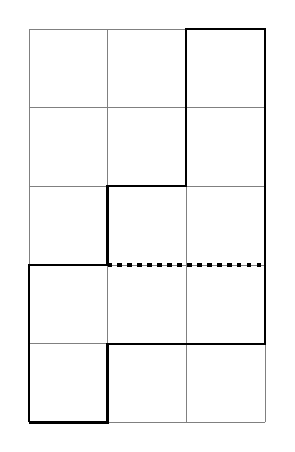
\begin{tikzpicture}
            \draw[help lines] (0,0) grid (3,5);
            \draw[thick] (0,0) -- (1,0) -- (1,1) -- (3,1) -- (3,5) --
                         (2,5) -- (2,3) -- (1,3) -- (1,2) -- (0,2) -- (0,0);
            \draw[ultra thick,dotted] (1,2) -- (3,2);
            \end{tikzpicture}
        \end{center}
	}

	\example
	{
		6
		0 0
		1 0
		1 1
		2 1
		2 2
		0 2
	}
	{
		NO
	}
    {
        I dette tilfælde er der ingen måde at dele øen i to kongruente
        polygoner.
        \begin{center}
            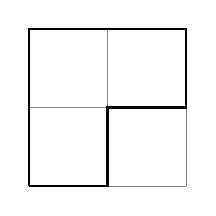
\begin{tikzpicture}
            \draw[help lines] (0,0) grid (2,2);
            \draw[thick] (0,0) -- (1,0) -- (1,1) --
                         (2,1) -- (2,2) -- (0,2) -- (0,0);
            \end{tikzpicture}
        \end{center}
    }

    \Scoring

    \begin{description}
        \item[Delopgave 1 (? point).] $4 \le N \le 100\,000$. Enhver linje,
            der deler polygonen vil dele polygonen i netop to stykker.
        \item[Delopgave 2 (? point).] $4 \le N \le 200$
        \item[Delopgave 3 (? point).] $4 \le N \le 4\,000$
        \item[Delopgave 4 (? point).] $4 \le N \le 100\,000$
    \end{description}

    \Constraints

    \begin{description}
        \item[Tidsbegrænsning:] 0.5 s.
        \item[Hukommelsesbegrænsning:] 256 MB.
    \end{description}

\end{document}
